%%%%%%%%%%%%%%%%%%%%%%%%%%%%%%%%%%%%%%%%%%%%%%%%%%%
% CHƯƠNG 4: THIẾT KẾ VÀ CHẾ TẠO HỆ THỐNG PHẦN CỨNG DRONE VÀ TRẠM MẶT ĐẤT
%%%%%%%%%%%%%%%%%%%%%%%%%%%%%%%%%%%%%%%%%%%%%%%%%%%
\section*{CHƯƠNG 4. THIẾT KẾ VÀ CHẾ TẠO HỆ THỐNG PHẦN CỨNG DRONE VÀ TRẠM MẶT ĐẤT}
\addcontentsline{toc}{section}{\numberline{}CHƯƠNG 4. THIẾT KẾ VÀ CHẾ TẠO HỆ THỐNG PHẦN CỨNG DRONE VÀ TRẠM MẶT ĐẤT}
\setcounter{section}{4}
\setcounter{subsection}{0}
\setcounter{figure}{0}
\setcounter{table}{0}

\subsection{Thiết kế phần cứng và cơ khí Drone}

Việc tự thiết kế bo mạch điều khiển bay Flight Controller (FC) giúp nâng cao khả năng làm chủ công nghệ nhúng, tối ưu hóa kích thước và sơ đồ chân (pinout) theo đúng nhu cầu sử dụng thực tế của hệ thống Drone cứu nạn, đồng thời loại bỏ các tính năng dư thừa của các bo mạch thương mại.

Sơ đồ cấu trúc phần cứng tổng quát và các kết nối ngoại vi của toàn bộ hệ thống Drone được mô tả trong Hình \ref{fig:so_do_khoi_he_thong}.

\begin{figure}[H]
    \centering
    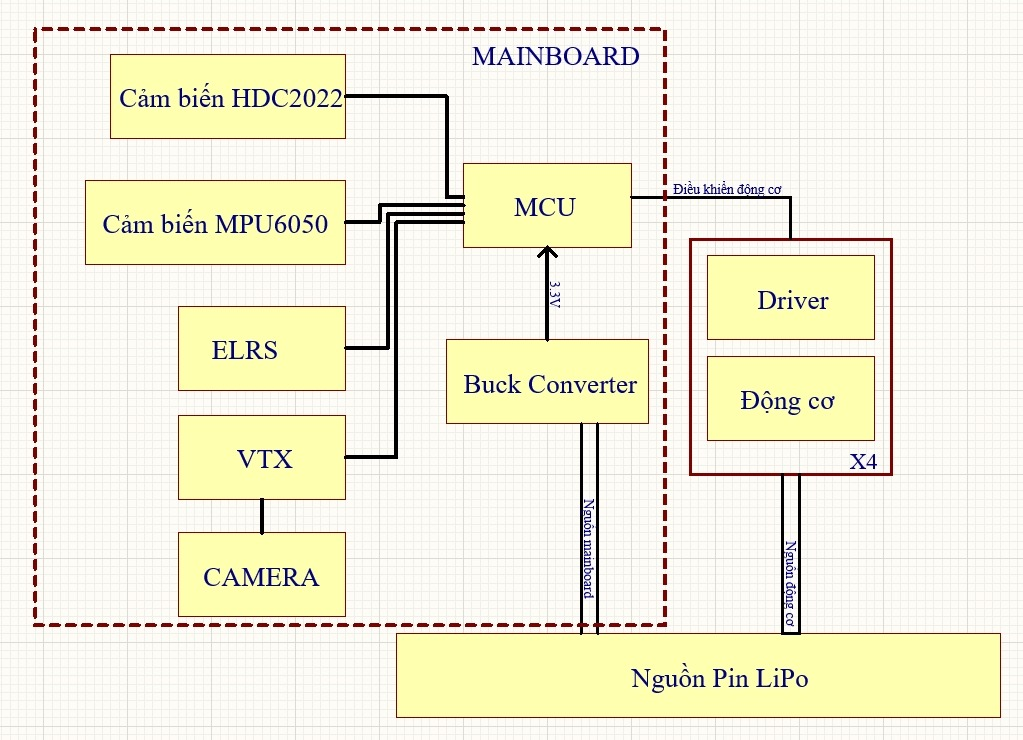
\includegraphics[width=0.85\textwidth]{Images/so_do_khoi_he_thong.jpg}
    \caption[Sơ đồ khối cấu trúc phần cứng và kết nối ngoại vi hệ thống Drone]{\bfseries\fontsize{12pt}{0pt}\selectfont Sơ đồ khối cấu trúc phần cứng và kết nối ngoại vi hệ thống Drone}
    \label{fig:so_do_khoi_he_thong}
\end{figure}

Hệ thống được chia làm hai khu vực chính:
\begin{itemize}
    \item \textbf{Bo mạch chính (Mainboard - Flight Controller):} Đóng vai trò là trung tâm xử lý dữ liệu và điều phối hoạt động bay. Tích hợp trên bo mạch bao gồm vi điều khiển (MCU) trung tâm kết nối trực tiếp với các cảm biến quán tính IMU MPU6050 (đọc vận tốc góc và gia tốc), cảm biến khí hậu HDC2022 (đo nhiệt độ và độ ẩm môi trường xung quanh), bộ thu sóng điều khiển ELRS (nhận lệnh từ tay phát) và bộ truyền hình ảnh VTX kết nối trực tiếp với camera FPV để truyền tải luồng video trực tuyến về trạm mặt đất. Một bộ hạ áp Buck Converter được tích hợp trực tiếp trên bo mạch để nhận điện áp cao từ pin LiPo và chuyển đổi thành nguồn sạch cấp cho MCU (qua bộ ổn áp LDO 3.3V) và các module cảm biến, thu phát sóng.
    \item \textbf{Hệ thống động lực ngoại vi:} Bao gồm bộ nguồn Pin LiPo dung lượng lớn để cung cấp năng lượng độc lập. Nguồn pin cấp trực tiếp cho 4 cụm Driver (ESC) và động cơ không chổi than, đồng thời dẫn tới ngõ vào nguồn của Mainboard. Vi điều khiển trung tâm (MCU) xuất 4 đường tín hiệu xung PWM chuyên dụng để điều khiển hoạt động đồng bộ của 4 động cơ thông qua các bộ ESC tương ứng.
\end{itemize}

\subsubsection{Thiết kế sơ đồ nguyên lý và Layout PCB Flight Controller}


Bo mạch điều khiển bay được thiết kế trên phần mềm Altium Designer xoay quanh vi điều khiển trung tâm STM32F103C8T6 (kiến trúc ARM Cortex-M3, hoạt động ở tần số 72\,MHz). Sơ đồ nguyên lý chi tiết được thiết kế chia làm hai bản vẽ chính:
\begin{itemize}
    \item \textbf{Bản vẽ nguồn chính và chuyển đổi nguồn (Hình \ref{fig:schematic_fc_power})}:
    \begin{itemize}
        \item \textit{Khối Power Main}: Sử dụng IC chuyển đổi nguồn dạng xung Buck TPS5450DDAR hiệu suất cao để chuyển đổi từ điện áp pin LiPo chính 12V xuống 5V. Đường vào được lọc nhiễu bởi tụ hóa C22 ($120\,\mu\text{F}/35\text{V}$) kết hợp tụ gốm C23 ($10\,\text{nF}$). Đầu ra sử dụng cuộn cảm L1 ($18\,\mu\text{H}$) kết hợp diode Schottky SS54 và các tụ lọc C26 ($220\,\mu\text{F}/10\text{V}$), C31 ($10\,\text{nF}$) để san phẳng điện áp ngõ ra 5V ổn định. Mạch phản hồi sử dụng cầu phân áp R5 ($18\,\text{k}\Omega$) và R10 ($5.6\,\text{k}\Omega$) để duy trì điện áp 5V chuẩn xác.
        \item \textit{Khối ổn áp tuyến tính 5V - 3.3V MCU}: Sử dụng IC AMS1117-3.3V để chuyển đổi từ nguồn 5V ổn định xuống 3.3V cấp cho vi điều khiển STM32 và các linh kiện logic nhạy cảm. Hệ thống tụ lọc đầu vào C27 ($22\,\mu\text{F}$), C28 ($100\,\text{nF}$) và đầu ra C29 ($100\,\text{nF}$), C30 ($22\,\mu\text{F}$) đảm bảo giảm thiểu tối đa nhiễu gợn sóng cao tần. LED D1 báo nguồn qua trở hạn dòng R9 ($1\,\text{k}\Omega$).
        \item \textit{Jack nguồn vào J2}: Sử dụng giắc DC5525 để nhận nguồn DC 12V từ pin 3S.
    \end{itemize}
    \item \textbf{Bản vẽ khối điều khiển và giao tiếp ngoại vi (Hình \ref{fig:schematic_fc_mcu})}:
    \begin{itemize}
        \item \textit{Khối MCU trung tâm}: Vi điều khiển STM32F103C8T6 với mạch Reset cứng (nút nhấn RST, trở kéo lên 10\,k$\Omega$, tụ lọc nhiễu 0.1\,$\mu$F), mạch dao động thạch anh ngoài 8\,MHz (CLOCK) sử dụng tụ lọc 22\,pF và mạch thạch anh thời gian thực 32.768\,kHz sử dụng tụ lọc 10\,pF.
        \item \textit{Khối cảm biến IMU MPU-6050}: Giao tiếp với MCU qua bus I2C (SCL, SDA) tích hợp các tụ lọc nguồn nhiễu C12, C13 (0.1\,$\mu$F).
        \item \textit{Khối bộ nhớ EEPROM 24LC256}: Lưu trữ các thông số hiệu chuẩn cảm biến và hệ số PID, kết nối qua bus I2C dùng chung với MPU-6050.
        \item \textit{Khối đo năng lượng (ĐO NL)}: Thiết kế mạch cầu phân áp gồm R8 ($27\,\text{k}\Omega$) và R12 ($10\,\text{k}\Omega$) để đo điện áp pin VBAT đưa về chân ADC của MCU.
        \item \textit{Khối kết nối ngoại vi}: Các giắc kết nối giao tiếp với mạch thu ELRS, mạch phát truyền hình ảnh VTX, và khối cảm biến khí tượng (AIR SENS) sử dụng cảm biến nhiệt độ - độ ẩm HDC2022DEPR qua I2C.
        \item \textit{Khối điều khiển động cơ (DRIVE A2212)}: Trích xuất các cổng PWM1 đến PWM4 từ Timer của STM32 cấp cho ESC điều khiển động cơ.
    \end{itemize}
\end{itemize}

\begin{figure}[H]
    \centering
    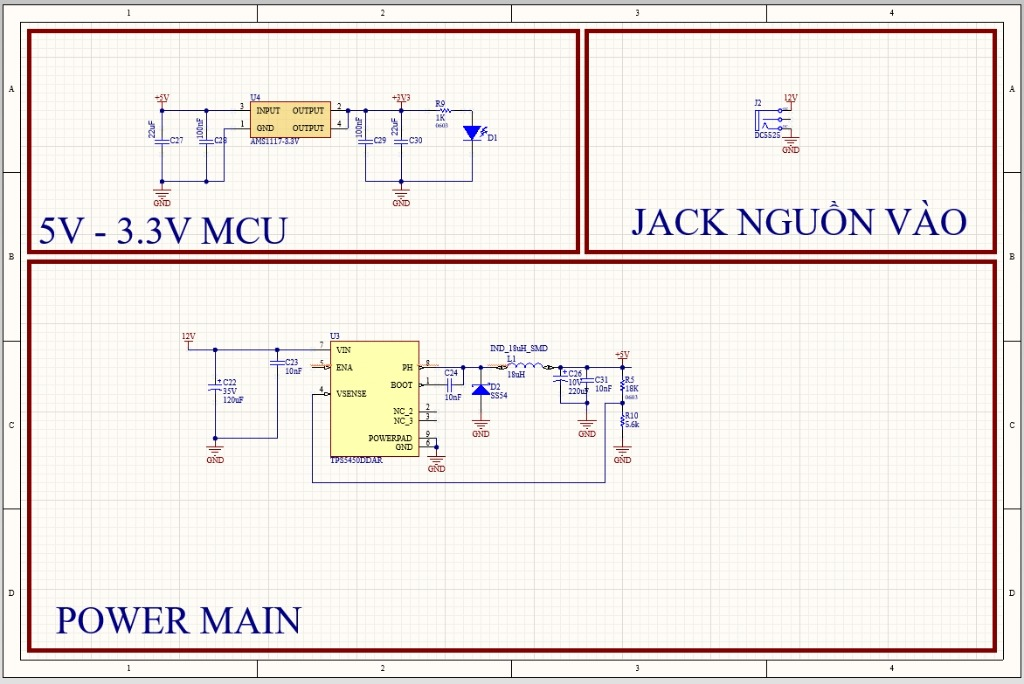
\includegraphics[width=0.95\textwidth]{Images/schematic_fc_power.jpg}
    \caption[Sơ đồ nguyên lý Flight Controller - Khối mạch nguồn chính]{\bfseries\fontsize{12pt}{0pt}\selectfont Sơ đồ nguyên lý Flight Controller - Khối mạch nguồn chính}
    \label{fig:schematic_fc_power}
\end{figure}

\begin{figure}[H]
    \centering
    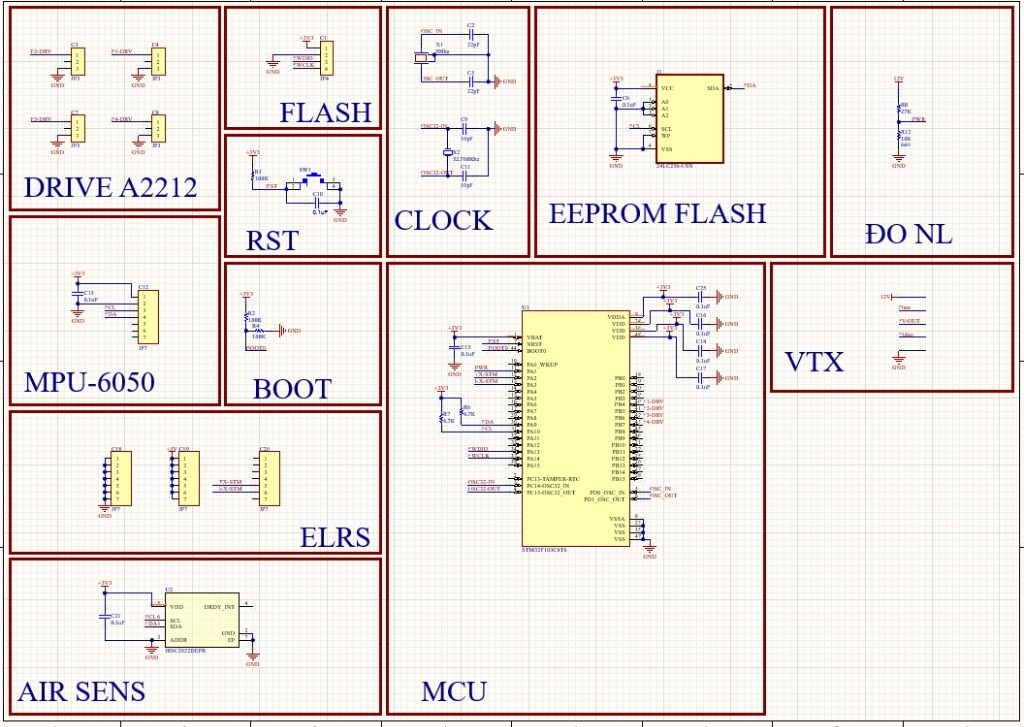
\includegraphics[width=0.95\textwidth]{Images/schematic_fc_mcu.jpg}
    \caption[Sơ đồ nguyên lý Flight Controller - Khối vi điều khiển và ngoại vi]{\bfseries\fontsize{12pt}{0pt}\selectfont Sơ đồ nguyên lý Flight Controller - Khối vi điều khiển và ngoại vi}
    \label{fig:schematic_fc_mcu}
\end{figure}

Layout PCB được thiết kế trên mạch 2 lớp (Double-sided PCB) với kích thước tiêu chuẩn 36\,x\,36\,mm, khoảng cách lỗ bắt ốc 30.5\,x\,30.5\,mm phù hợp với hầu hết các khung sườn Drone phổ thông. Chi tiết thiết kế Layout PCB và phối cảnh 3D của bo mạch Flight Controller được mô tả trong Hình \ref{fig:pcb_layout_3d}:
\begin{itemize}
    \item \textbf{Phối cảnh 3D}: Bo mạch được thiết kế dưới dạng hình bát giác đều cách điệu, bo tròn các góc để tăng tính cơ khí bền bỉ. Mạch khoét lỗ rỗng lớn ở tâm để tối ưu hóa việc phân bố trọng lượng, đi dây động lực xuyên qua sườn Drone và hỗ trợ tản nhiệt. Các linh kiện SMD được phân bố đồng đều, các cổng kết nối ngoại vi (như chân cắm nạp SWD, I2C, UART) được sắp xếp ở các mép cạnh giúp người vận hành dễ dàng thao tác cắm dây.
    \item \textbf{Lớp Top Layer (Mặt trên)}: Đi dây các đường nguồn chính với bề rộng lớn (VBAT, 5V, 3.3V) để tránh sụt áp và chịu tải dòng điện tốt. Các linh kiện công suất như IC TPS5450, cuộn cảm L1, tụ hóa C22 được ưu tiên đặt ở lớp trên. Các pad kết nối lớn ở viền mạch hỗ trợ cấp nguồn cho mạch truyền hình ảnh VTX và ESC.
    \item \textbf{Lớp Bottom Layer (Mặt dưới)}: Chứa các đường tín hiệu logic, I2C, UART kết nối chéo thông qua các lỗ via. Việc phân tách đường tín hiệu sang lớp Bottom giúp tránh hiện tượng nhiễu từ trường phát sinh từ các linh kiện công suất lớn ở lớp Top. Toàn bộ phần diện tích trống ở lớp dưới được phủ đồng GND để tối ưu khả năng khử nhiễu.
\end{itemize}

\begin{figure}[H]
    \centering
    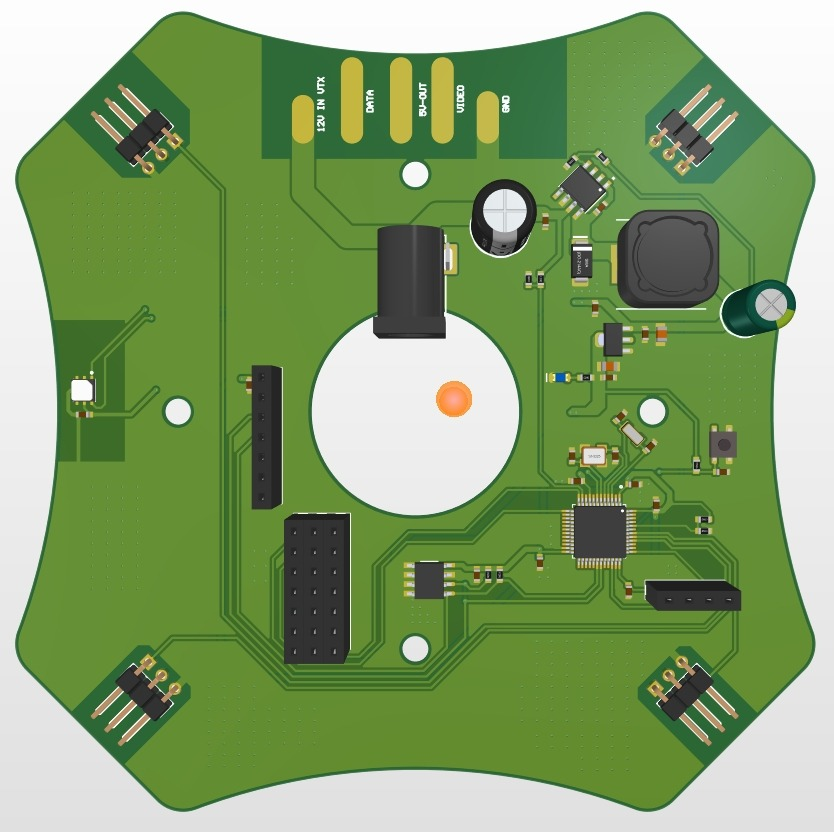
\includegraphics[width=0.31\textwidth]{Images/layout_pcb_fc_3d.jpg} \hfill
    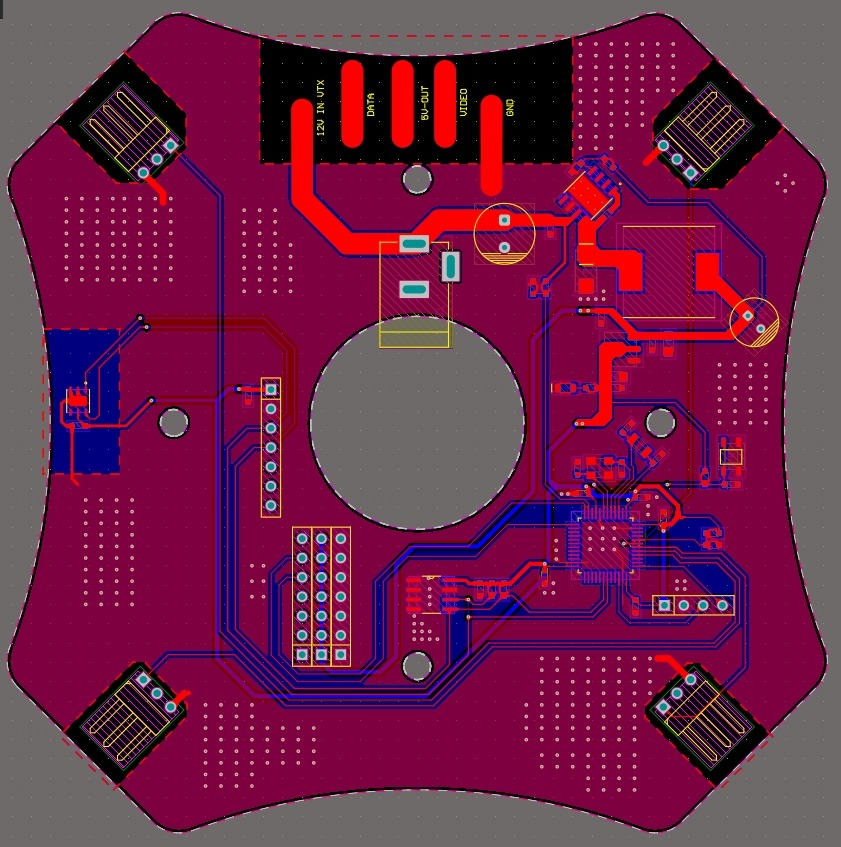
\includegraphics[width=0.31\textwidth]{Images/layout_pcb_fc_top.jpg} \hfill
    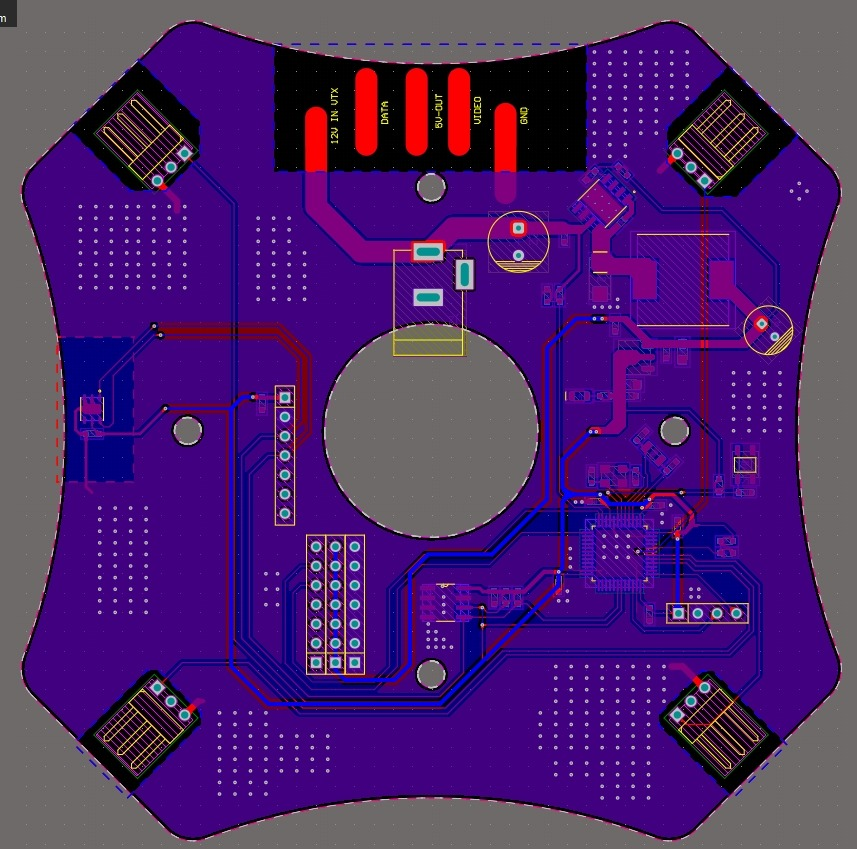
\includegraphics[width=0.31\textwidth]{Images/layout_pcb_fc_bottom.jpg}
    \caption[Thiết kế Layout PCB và phối cảnh 3D Flight Controller]{\bfseries\fontsize{12pt}{0pt}\selectfont Thiết kế Layout PCB và phối cảnh 3D Flight Controller: Phối cảnh 3D (trái), Layout lớp Top (giữa) và Layout lớp Bottom (phải)}
    \label{fig:pcb_layout_3d}
\end{figure}

\subsubsection{Thiết kế mạch nguồn logic và cầu phân áp đo pin}

Do các động cơ không chổi than khi thay đổi tốc độ đột ngột sẽ tạo ra các xung nhiễu điện áp ngược rất lớn trên đường nguồn chính VBAT, việc thiết kế hệ thống nguồn cấp điện cho các chip logic nhạy cảm (MCU, IMU) yêu cầu độ ổn định cực kỳ nghiêm ngặt. Sơ đồ mạch nguồn hạ áp phân tầng sử dụng chip nguồn xung Buck TPS5450DDAR kết hợp chip ổn áp tuyến tính LDO AMS1117-3.3V được thể hiện chi tiết tại Hình \ref{fig:schematic_fc_power}.

Hệ thống nguồn bao gồm hai tầng chính:
\begin{enumerate}
    \item \textbf{Tầng hạ áp Buck (TPS5450-5.0)}: Sử dụng IC hạ áp Buck chuyển mạch TPS5450DDAR của hãng Texas Instruments. Với tần số chuyển mạch cao 500\,kHz và dòng điện ngõ ra tối đa đạt 5A, TPS5450 cung cấp nguồn 5V mạnh mẽ và hiệu suất cao (>90\%) cho các tải lớn như bộ thu sóng ELRS, camera FPV, gimbal và cảm biến ngoại vi. Tụ hóa ngõ vào C22 ($120\,\mu\text{F}/35\text{V}$) triệt tiêu các xung áp sụt đột ngột, trong khi cuộn cảm L1 ($18\,\mu\text{H}$), diode SS54 và tụ hóa ngõ ra C26 ($220\,\mu\text{F}/10\text{V}$) tạo bộ lọc thông thấp làm mịn điện áp đầu ra.
    \item \textbf{Tầng ổn áp tuyến tính LDO (AMS1117-3.3)}: Ổn áp từ nguồn 5.0V trung gian xuống 3.3V cấp cho MCU STM32 và cảm biến MPU6050. Mạch LDO cung cấp điện áp cực kỳ sạch, triệt tiêu các nhiễu gợn sóng cao tần (high-frequency ripple) phát sinh từ mạch Buck.
\end{enumerate}

Để giám sát dung lượng pin nhằm đưa ra cảnh báo hạ cánh an toàn, một mạch cầu phân áp được thiết kế nối từ cực dương pin VBAT về chân ADC (PA4) của MCU:
\begin{equation}
    V_{ADC} = V_{BAT} \cdot \frac{R_2}{R_1 + R_2}
\end{equation}
Với giá trị điện trở lựa chọn $R_1 = 10\,k\Omega$ và $R_2 = 3.3\,k\Omega$, điện áp pin lớn nhất $12.6V$ được hạ xuống mức an toàn $3.12V$, nằm hoàn toàn trong dải đo tuyến tính của bộ ADC 12-bit trên vi điều khiển STM32 (0V - 3.3V).

\subsubsection{Lắp ráp cơ khí và hệ thống động lực}

Khung sườn Drone được sử dụng là khung Carbon FPV F450 chịu lực tốt và trọng lượng nhẹ. Hệ thống động lực được lựa chọn dựa trên sự tính toán cân bằng lực đẩy tối ưu:
\begin{itemize}
    \item \textbf{Động cơ}: A2212 1000KV không chổi than, cung cấp lực đẩy tối đa khoảng 850g mỗi động cơ ở mức ga 100\% khi đi kèm cánh quạt 1045. Tổng lực đẩy tối đa của 4 động cơ đạt 3400g.
    \item \textbf{Trọng lượng Drone}: Tổng trọng lượng cất cánh (bao gồm pin Lipo, camera FPV, mạch FC và khung sườn) là 950g. Tỷ số lực đẩy trên trọng lượng (Thrust-to-Weight Ratio) đạt:
    \begin{equation}
        \text{Tỷ lệ Lực đẩy/Trọng lượng} = \frac{3400g}{950g} \approx 3.58
    \end{equation}
    Tỉ số này lớn hơn ngưỡng an toàn tối thiểu 2.0 rất nhiều, đảm bảo Drone có khả năng gia tốc cực tốt, kháng gió mạnh và hoạt động ổn định ở môi trường ngoài trời.
    \item \textbf{Pin nguồn}: Pin LiPo 3S 11.1V 2200mAh dòng xả 45C cho phép cung cấp dòng điện liên tục lên tới $2.2 \times 45 = 99A$, đáp ứng hoàn hảo nhu cầu dòng điện tức thời cực đại khi cả 4 ESC hoạt động hết công suất.
\end{itemize}

Hình dạng thực tế của mô hình Drone sau khi lắp ráp cơ khí hoàn chỉnh và tích hợp bo mạch điều khiển bay Flight Controller được thể hiện trong Hình \ref{fig:drone_lap_rap_thuc_te}.

\begin{figure}[H]
    \centering
    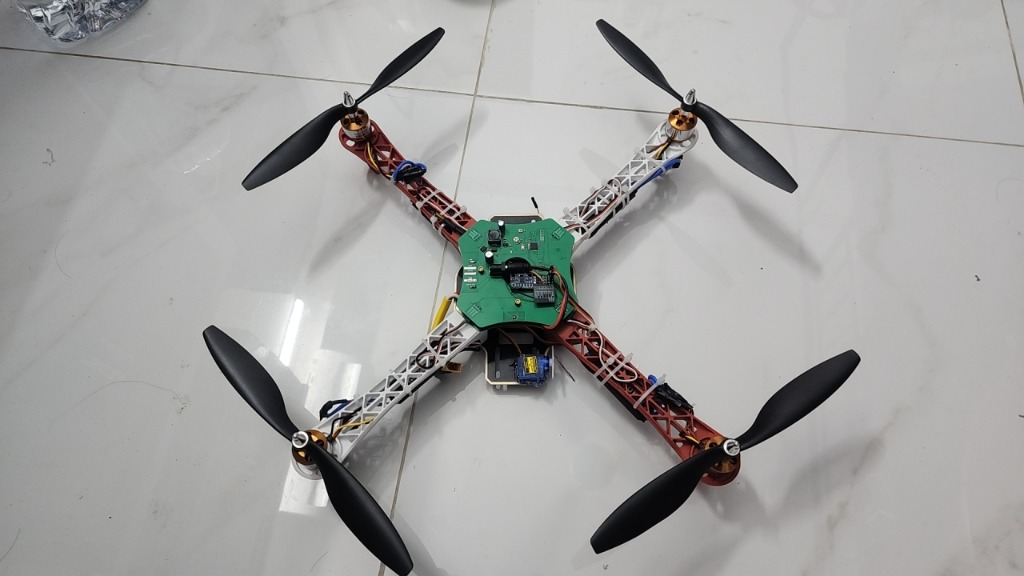
\includegraphics[width=0.65\textwidth]{Images/agent/drone_thuc_te.jpg}
    \caption[Mô hình thực tế hệ thống Drone cứu hộ hoàn thiện]{\bfseries\fontsize{12pt}{0pt}\selectfont Mô hình thực tế hệ thống Drone cứu hộ hoàn thiện}
    \label{fig:drone_lap_rap_thuc_te}
\end{figure}

\subsection{Lập trình phần mềm nhúng (Firmware Flight Controller)}

Firmware điều khiển bay được lập trình bằng ngôn ngữ C++ trực tiếp trên nền tảng Bare-metal (không sử dụng hệ điều hành thời gian thực RTOS) để tối ưu hóa tốc độ thực thi và loại bỏ độ trễ do chuyển đổi ngữ cảnh tác vụ (task context switching), đồng thời có tham khảo cơ chế lập lịch vòng lặp từ dự án mã nguồn mở Betaflight \cite{betaflight2024}.

\subsubsection{Kiến trúc vòng lặp điều khiển chính thời gian thực tần số 250Hz}

Độ ổn định của thiết bị bay phụ thuộc quyết định vào tính ổn định thời gian thực của vòng lặp điều khiển chính. Chu kỳ vòng lặp được thiết lập cố định ở tần số 250\,Hz (tương đương chu kỳ lấy mẫu $T_s = 4000\mu s$). Lưu đồ thuật toán khởi động và trạng thái của máy trạng thái (FSM) trong firmware được trình bày trong Hình \ref{fig:luu_do_fsm_boot}.

\begin{figure}[H]
    \centering
    \resizebox{0.85\textwidth}{!}{
    \begin{tikzpicture}[
        arrow/.style={-Latex, thick, draw=black},
        state/.style={rectangle, draw=black, fill=white, thick, minimum width=5.2cm, minimum height=1.0cm, align=center, rounded corners=3pt, font=\fontsize{8.5pt}{10pt}\selectfont},
        errorstate/.style={rectangle, draw=black, fill=gray!10, thick, minimum width=5.0cm, minimum height=1.2cm, align=center, rounded corners=3pt, font=\fontsize{8.5pt}{10pt}\selectfont}
    ]
        % Entry Point
        \node[circle, fill=black, inner sep=2.5pt, label=above:{\fontsize{8.5pt}{10pt}\selectfont Khởi động hệ thống (Power On)}] (start) at (0, 5.8) {};

        % States (Main path)
        \node[state] (boot) at (0, 4.6) {\textbf{STARTUP\_BOOT}\\Tải cấu hình từ lưu trữ};
        \node[state] (imu_init) at (0, 3.0) {\textbf{STARTUP\_IMU\_INIT}\\Khởi tạo cảm biến MPU6050};
        \node[state] (gyro_calib) at (0, 1.4) {\textbf{STARTUP\_GYRO\_CALIB}\\Hiệu chuẩn Gyroscope (1000 mẫu)};
        \node[state] (rc_check) at (0, -0.2) {\textbf{STARTUP\_RC\_CHECK}\\Kiểm tra kết nối và tay ga RC};
        \node[state] (acc_check) at (0, -1.8) {\textbf{STARTUP\_ACC\_CHECK}\\Kiểm tra gia tốc tĩnh ($g \approx 1.0$)};
        \node[state] (esc_check) at (0, -3.4) {\textbf{STARTUP\_ESC\_CHECK}\\Kiểm tra cờ calib ESC/Accel};
        \node[state, fill=gray!2] (ready) at (0, -5.0) {\textbf{STARTUP\_READY}\\Sẵn sàng bay (Vòng lặp chính)};

        % Error State
        \node[errorstate] (error) at (9.5, -1.0) {\textbf{STARTUP\_ERROR}\\Dừng động cơ khẩn cấp\\(Nháy chớp LED báo lỗi)};

        % Transitions (Main path)
        \draw[arrow] (start) -- (boot.north);
        \draw[arrow] (boot.south) -- (imu_init.north);
        
        \draw[arrow] (imu_init.south) -- node[right, font=\fontsize{7.5pt}{7.5pt}\selectfont] {Thành công} (gyro_calib.north);
        
        \draw[arrow] (gyro_calib.south) -- node[right, font=\fontsize{7.5pt}{7.5pt}\selectfont] {Thành công} (rc_check.north);
        
        \draw[arrow] (rc_check.south) -- node[right, font=\fontsize{7.5pt}{7.5pt}\selectfont] {Thành công} (acc_check.north);
        
        \draw[arrow] (acc_check.south) -- node[right, font=\fontsize{7.5pt}{7.5pt}\selectfont] {Thành công} (esc_check.north);
        
        \draw[arrow] (esc_check.south) -- node[right, font=\fontsize{7.5pt}{7.5pt}\selectfont] {Hoàn thành} (ready.north);

        % Gyro Self-loop
        \draw[arrow] (gyro_calib.west) .. controls ++(-1.6, 0.4) and ++(-1.6, -0.4) .. (gyro_calib.west) 
            node[pos=0.5, left, font=\fontsize{7.5pt}{7.5pt}\selectfont, align=center] {Phát hiện rung lắc\\(Thử lại $<$ 5 lần)};

        % Coordinates for error anchors
        \coordinate (err_1) at ([yshift=0.4cm]error.west);
        \coordinate (err_2) at ([yshift=0.15cm]error.west);
        \coordinate (err_3) at ([yshift=-0.1cm]error.west);
        \coordinate (err_4) at ([yshift=-0.35cm]error.west);

        % Error Transitions (using explicit segments)
        \draw[arrow] (imu_init.east) -- (6.7, 3.0) -- (6.7, -0.6) -- (err_1);
        \draw[arrow] (gyro_calib.east) -- (6.5, 1.4) -- (6.5, -0.85) -- (err_2);
        \draw[arrow] (rc_check.east) -- (6.3, -0.2) -- (6.3, -1.1) -- (err_3);
        \draw[arrow] (acc_check.east) -- (6.5, -1.8) -- (6.5, -1.35) -- (err_4);

        % Labels for error transitions (placed to the left of the vertical lines)
        \node[above right, font=\fontsize{7.5pt}{7.5pt}\selectfont, align=left, inner sep=2pt] at (imu_init.east) {Lỗi kết nối I2C\\(ERR\_IMU\_INIT\_FAIL)};
        \node[above right, font=\fontsize{7.5pt}{7.5pt}\selectfont, align=left, inner sep=2pt] at (gyro_calib.east) {Rung lắc quá 5 lần\\(ERR\_GYRO\_CALIB\_MOVING)};
        \node[above right, font=\fontsize{7.5pt}{7.5pt}\selectfont, align=left, inner sep=2pt] at (rc_check.east) {Mất sóng/Ga cao/Lệch cần\\(ERR\_RC\_CENTER / ERR\_THROTTLE)};
        \node[above right, font=\fontsize{7.5pt}{7.5pt}\selectfont, align=left, inner sep=2pt] at (acc_check.east) {Lệch trục gia tốc tĩnh\\(ERR\_ACC\_VALIDATION\_FAIL)};

        % CLI Command Reset
        \draw[arrow] (error.east) -- (13.0, -1.0) -- (13.0, 4.6) -- (boot.east)
            node[pos=0.25, right, font=\fontsize{7.5pt}{7.5pt}\selectfont, align=left] {Nhận lệnh 'c' qua CLI\\(Reset trạng thái lỗi)};

    \end{tikzpicture}
    }
    \caption[Sơ đồ máy trạng thái khởi động FSM Boot của Drone]{Sơ đồ máy trạng thái khởi động FSM Boot của Drone}
    \label{fig:luu_do_fsm_boot}
\end{figure}

Quy trình hoạt động trong vòng lặp chính của firmware bao gồm các bước tuần tự được đồng bộ thời gian khắt khe:
\begin{enumerate}
    \item \textbf{Chờ đồng bộ}: Sử dụng bộ đếm thời gian hệ thống High-Resolution Microsecond Timer để đo đạc chính xác thời điểm bắt đầu vòng lặp mới, đảm bảo đúng chu kỳ $4000\mu s$.
    \item \textbf{Đọc dữ liệu IMU}: Giao tiếp bus I2C đọc các thanh ghi dữ liệu thô của Gyroscope và Accelerometer trên MPU6050.
    \item \textbf{Ước lượng tư thế}: Thực thi thuật toán bộ lọc bù để tính toán góc nghiêng hiện tại (Roll, Pitch, Yaw).
    \item \textbf{Giải mã lệnh điều khiển}: Đọc luồng dữ liệu CRSF từ bộ thu sóng để cập nhật giá trị Setpoint mong muốn của người điều khiển.
    \item \textbf{Tính toán PID song song}: Chạy đồng thời 3 bộ điều khiển PID kép (Cascade PID) cho 3 trục bay để tính toán giá trị hiệu chỉnh lực nâng.
    \item \textbf{Trộn ga và xuất xung PWM}: Trộn giá trị điều khiển PID với tay ga chính (Throttle) để tính toán chu kỳ nhiệm vụ PWM cấp cho từng động cơ theo cấu hình Quad-X.
\end{enumerate}

\subsubsection{Giao tiếp Software I2C tốc độ cao và Đọc/Ghi EEPROM}

Do cảm biến MPU6050 và EEPROM 24LC256 nằm chung trên bus I2C, việc quản lý truyền thông không được để xảy ra hiện tượng nghẽn bus làm gián đoạn vòng lặp 250\,Hz. Đồ án xây dựng driver Software I2C (Bit-banging) sử dụng trực tiếp các thanh ghi cấu hình IO tốc độ cao của STM32 để đạt tần số clock truyền thông lên tới 400\,kHz (Fast Mode).

Bộ nhớ EEPROM 24LC256 được phân vùng để lưu trữ:
\begin{itemize}
    \item Giá trị hiệu chuẩn điểm không cảm biến (Gyro Offset, Accel Calibration).
    \item Các hệ số điều khiển PID ($K_p, K_i, K_d$) của 3 trục Roll, Pitch, Yaw.
\end{itemize}
Khi cấp nguồn, MCU sẽ đọc cấu hình từ EEPROM để khởi tạo hệ thống. Khi người dùng thay đổi PID từ trạm mặt đất, các tham số mới sẽ được ghi đè vào EEPROM một cách an toàn.

\subsubsection{Giải mã CRSF và Cơ chế an toàn Failsafe}

Giao thức CRSF từ bộ thu ELRS truyền về MCU qua cổng UART dưới dạng các khung tin nhị phân. Firmware sử dụng kỹ thuật ngắt nhận dữ liệu UART kết hợp bộ đệm vòng (Ring Buffer) để tránh làm mất mát dữ liệu khi MCU đang bận tính toán PID.

Mỗi khung dữ liệu nhận được chứa 11-bit giá trị tay ga cho mỗi kênh (từ 172 đến 1811, tương ứng thời gian xung từ $988\mu s$ đến $2012\mu s$). Hàm giải mã trích xuất kênh điều khiển và thực hiện chuyển đổi tuyến tính sang góc đặt Setpoint nghiêng từ $-30^\circ$ đến $+30^\circ$.

Để đảm bảo an toàn tuyệt đối cho người vận hành và thiết bị bay, cơ chế an toàn **Failsafe** được xây dựng chặt chẽ:
\begin{itemize}
    \item Firmware liên tục giám sát khoảng thời gian nhận được gói tin CRSF thành công gần nhất.
    \item Nếu quá thời gian $T_{lost} = 500\mu s$ mà không nhận được tín hiệu điều khiển mới từ bộ thu (mất sóng, hết pin tay phát), hệ thống sẽ tự động kích hoạt chế độ Failsafe: ngắt kích hoạt động cơ ngay lập tức (Disarm) để tránh hiện tượng Drone tự bay mất kiểm soát (Fly-away).
\end{itemize}

\subsection{Thiết kế phần mềm điều phối trạm mặt đất}

Phần mềm trạm mặt đất (GCS) được phát triển bằng ngôn ngữ Python sử dụng thư viện giao diện đồ họa PyQt5, đóng vai trò nhận luồng video thời gian thực từ đầu thu FPV, chạy các mô hình AI phát hiện sự kiện cứu hộ và tương tác với người vận hành.

\subsubsection{Kiến trúc hệ thống điều phối đa luồng (Multi-threading)}

Để đảm bảo giao diện đồ họa GUI hoạt động mượt mà và không bị giật lag khi đang thực hiện các phép toán nhận diện học sâu cực kỳ nặng, kiến trúc phần mềm được thiết kế phân lớp đa luồng như mô tả trong Hình \ref{fig:luong_phan_mem_gui}.

\begin{figure}[H]
    \centering
    \begin{tikzpicture}[
        node distance=1.2cm and 1.2cm,
        thread/.style={rectangle, draw=black, fill=white, thick, rounded corners, minimum width=3.4cm, minimum height=1.1cm, align=center, font=\bfseries\fontsize{9pt}{11pt}\selectfont},
        data/.style={ellipse, draw=black, fill=white, thick, minimum width=2.4cm, minimum height=0.9cm, align=center, font=\fontsize{8pt}{9pt}\selectfont},
        queue/.style={rectangle, draw=black, fill=white, thick, minimum width=2.6cm, minimum height=0.9cm, align=center, font=\fontsize{8pt}{9pt}\selectfont},
        io/.style={rectangle, draw=black, fill=white, thick, rounded corners=2pt, minimum width=2.4cm, minimum height=0.9cm, align=center, font=\fontsize{8pt}{9pt}\selectfont},
        arrow/.style={-Latex, thick, draw=black},
        signal/.style={-Latex, dashed, thick, draw=black, text=black, font=\fontsize{7.5pt}{8.5pt}\selectfont}
    ]

        % Grid Layout Configuration (Monochrome)
        % Column 1: x = 0
        % Column 2: x = 4.2
        % Column 3: x = 8.4
        % Column 4: x = 12.6
        
        % Row 1: y = 3
        \node[io] (camera) at (0,3) {Camera FPV\\(Dữ liệu video thô)};
        \node[thread] (video_thread) at (4.2,3) {Luồng nhận video\\(Sử dụng OpenCV)};
        \node[queue] (frame_queue) at (8.4,3) {Hàng đợi khung hình\\(Thread-safe Queue)};
        \node[thread] (inference_thread) at (12.6,3) {Luồng suy luận AI\\(YOLOv8 \& Dung hợp)};
        
        % Row 2: y = 0
        \node[io] (serial_port) at (0,0) {Bộ thu ELRS\\(Kết nối UART / USB)};
        \node[thread] (serial_thread) at (4.2,0) {Luồng nhận Telemetry\\(Giải mã dữ liệu Serial)};
        \node[thread] (gui_thread) at (8.4,0) {Luồng giao diện GUI\\(Luồng chính PyQt5)};
        \node[data] (target_mgr) at (12.6,0) {Bộ quản lý mục tiêu\\\& Khóa bám};
        
        % Row 3: y = -2
        \node[io] (operator) at (8.4,-2) {Màn hình trạm GCS\\(Giám sát \& Điều khiển)};

        % Connectors
        \draw[arrow] (camera) -- (video_thread);
        \draw[arrow] (video_thread) -- node[above, font=\fontsize{8pt}{9pt}\selectfont] {30 FPS} (frame_queue);
        \draw[arrow] (frame_queue) -- (inference_thread);
        
        \draw[arrow] (serial_port) -- (serial_thread);
        
        % Signals to GUI Thread (Rerouted with explicit label nodes to guarantee no overlap)
        \draw[signal] (inference_thread.south) -- ++(0,-0.25) -| ($(gui_thread.north east)-(0.4,0)$);
        \node[align=center, font=\fontsize{7.5pt}{8.5pt}\selectfont] at (10.7, 1.75) {Tín hiệu PyQt\\(Khung hình, Khung xương,\\Danger Score)};
            
        \draw[signal] (serial_thread.north) -- ++(0,0.25) -| ($(gui_thread.north west)+(0.4,0)$);
        \node[align=center, font=\fontsize{7.5pt}{8.5pt}\selectfont] at (5.8, 1.25) {Tín hiệu PyQt\\(Góc nghiêng,\\Điện áp pin)};
        
        \draw[arrow] (gui_thread) -- (operator);
        
        % Target Manager bidirectional connection
        \draw[arrow] ($(gui_thread.east)+(0,0.15)$) -- ($(target_mgr.west)+(0,0.15)$);
        \draw[arrow] ($(target_mgr.west)-(0,0.15)$) -- ($(gui_thread.east)-(0,0.15)$);

    \end{tikzpicture}
    \caption[Sơ đồ kiến trúc xử lý đa luồng tại trạm mặt đất GCS]{\bfseries\fontsize{12pt}{0pt}\selectfont Sơ đồ kiến trúc xử lý đa luồng tại trạm mặt đất GCS}
    \label{fig:luong_phan_mem_gui}
\end{figure}

Các luồng xử lý chạy song song độc lập tương tác qua cơ chế tín hiệu (Signals/Slots):
\begin{enumerate}
    \item \textbf{Luồng chính (GUI Thread)}: Đảm nhận việc vẽ giao diện người dùng, hiển thị khung hình video và tương tác nút nhấn.
    \item \textbf{Luồng nhận dữ liệu video (Video Ingestion Thread)}: Kết nối với camera FPV hoặc card capture USB để bắt các khung hình thô (raw frames) ở tốc độ 30 FPS bằng OpenCV, đẩy khung hình vào hàng đợi trung gian (Frame Queue).
    \item \textbf{Luồng suy luận AI (Inference Thread)}: Lấy khung hình từ Frame Queue, đẩy qua bộ Detector tích hợp 3 mô hình YOLO (YOLOv8-Rescue, YOLOv8-Posture, YOLOv8-Pose), thực hiện thuật toán dung hợp suy luận và gửi kết quả khung hình đã vẽ bounding box cùng tọa độ keypoints về GUI Thread.
    \item \textbf{Luồng Telemetry (Serial Communication Thread)}: Giao tiếp nối tiếp với mạch phát ELRS để nhận dữ liệu trạng thái Drone (điện áp pin, góc nghiêng thực tế) gửi ngược từ Drone về.
\end{enumerate}

\subsubsection{Bộ quản lý mục tiêu (Target Manager) và khóa mục tiêu (Focus Lock)}

Trong các tình huống giám sát đám đông hoặc khu vực thiên tai lớn, nhiều đối tượng có thể xuất hiện đồng thời trong một khung hình. Hệ thống xây dựng module **Target Manager** để theo dõi và quản lý định danh (ID) của từng mục tiêu:
\begin{itemize}
    \item Sử dụng thuật toán theo dõi đối tượng đa mục tiêu **ByteTrack** để gán ID duy nhất cho từng người phát hiện được dựa trên sự tương đồng về đặc trưng và khoảng cách giao nhau IoU (Intersection over Union) giữa các khung hình liên tiếp.
    \item Người vận hành có thể click chọn trực tiếp một mục tiêu cụ thể trên màn hình để kích hoạt cơ chế **Focus Lock** (Khóa nét tiêu điểm). Khi khóa nét, hệ thống sẽ tập trung tài nguyên tính toán để phân tích chi tiết tư thế keypoints và cử chỉ động cho duy nhất đối tượng đó, đồng thời gửi lệnh điều khiển gimbal camera quay bám đuổi mục tiêu được chọn.
\end{itemize}

\subsubsection{Giao diện tương tác và Hệ thống phím điều khiển của người vận hành}

Để đảm bảo khả năng phản ứng nhanh và linh hoạt của người vận hành trạm mặt đất trong các tình huống cứu nạn phức tạp, hệ thống thiết lập một giao diện tương tác tích hợp cho phép điều khiển và can thiệp trực tiếp bằng bàn phím và chuột. Các chức năng tương tác cốt lõi của người vận hành bao gồm:
\begin{itemize}
    \item \textbf{Phím quyết định của người vận hành (Operator Decisions)}:
    \begin{itemize}
        \item Phím \texttt{C} (Confirmed): Người vận hành chủ động xác nhận đối tượng đang khóa nét (Focus Target) thực sự là nạn nhân cần cứu trợ. Hành động này bỏ qua các đánh giá tự động và ngay lập tức lưu thông tin sự kiện kèm media.
        \item Phím \texttt{F} (False Alarm): Đánh dấu đối tượng được phát hiện là báo động giả. Hệ thống sẽ tự động hủy trạng thái nguy hiểm của đối tượng và xóa các file hình ảnh/video liên quan để giải phóng bộ nhớ.
        \item Phím \texttt{T} (Track More): Đánh dấu yêu cầu tiếp tục theo dõi tăng cường đối tượng này để thu thập thêm thông tin.
    \end{itemize}
    \item \textbf{Phím quản lý vùng giám sát nguy hiểm (ROI Controls)}:
    \begin{itemize}
        \item Phím \texttt{O}: Bật hoặc tắt tính năng giám sát vùng ROI.
        \item Phím \texttt{E}: Kích hoạt chế độ vẽ vùng nguy hiểm bằng cách click chuột để tạo các điểm đỉnh đa giác polygon trên màn hình.
        \item Phím \texttt{X}: Xóa bỏ hoàn toàn các cấu hình vùng ROI hiện tại.
    \end{itemize}
    \item \textbf{Phím thay đổi giao diện hiển thị (Display Controls)}:
    \begin{itemize}
        \item Giữ phím \texttt{Tab}: Hiển thị lớp phủ bảng thông số chấm điểm chi tiết (Overlay Panel) của mục tiêu đang chọn.
        \item Phím \texttt{P}: Bật hoặc tắt hiển thị khung xương 17 khớp (Skeleton).
        \item Phím \texttt{B}: Bật hoặc tắt thước ngắm chữ thập trung tâm (Crosshair) để hỗ trợ điều khiển camera bám đuổi.
    \end{itemize}
    \item \textbf{Phím điều phối hệ thống chung}:
    \begin{itemize}
        \item Phím \texttt{N}: Chuyển đổi khóa nét (Focus Lock) sang mục tiêu tiếp theo xuất hiện trong khung hình.
        \item Phím \texttt{S}: Khóa tiêu điểm nhanh vào đối tượng có Danger Score cao nhất.
        \item Phím \texttt{W}: Force refresh - yêu cầu cập nhật tức thời dữ liệu thời tiết tại trạm.
        \item Phím \texttt{A}: Mở cửa sổ Tkinter liệt kê danh sách nhật ký các sự kiện đã ghi nhận.
        \item Phím \texttt{R}: Xuất báo cáo HTML tức thời tại thời điểm hiện tại.
        \item Phím \texttt{Q} hoặc \texttt{Esc}: Lưu toàn bộ nhật ký sự kiện, tự động xuất báo cáo HTML hoàn chỉnh ra thư mục \texttt{reports/} và thoát an toàn khỏi chương trình.
    \end{itemize}
\end{itemize}

\subsubsection{Bộ ghi nhật ký sự kiện cứu hộ và Tự động xuất báo cáo HTML}

Khi giá trị điểm nguy cấp Danger Score của một mục tiêu vượt ngưỡng $DS \ge 85$ (xác nhận trạng thái khẩn cấp), phân hệ **Event Logger** sẽ tự động thực hiện:
\begin{enumerate}
    \item Trích xuất tọa độ GPS của Drone tại thời điểm phát hiện sự kiện (lấy từ dữ liệu Telemetry).
    \item Chụp ảnh cắt cảnh (snapshot) đối tượng nạn nhân từ luồng video, khoanh vùng khung đỏ và lưu ảnh vào thư mục sự kiện.
    \item Ghi nhận sự kiện vào tệp nhật ký \texttt{rescue\_events.csv} bao gồm các trường thông tin: \texttt{EventID, TimeStamp, Latitude, Longitude, DangerScore, PostureStatus}.
\end{enumerate}

Sau khi kết thúc chuyến bay tuần tra cứu nạn, module **Report Generator** sẽ tự động phân tích tệp CSV và ảnh chụp để xuất ra một báo cáo sự nghiệp cứu hộ hoàn chỉnh dưới định dạng tệp HTML chuyên nghiệp. Báo cáo này bao gồm biểu đồ trực quan hóa số lượng nạn nhân theo thời gian, bản đồ phân bố các vị trí phát hiện nạn nhân và bảng danh sách chi tiết kèm ảnh chụp cận cảnh từng trường hợp, giúp lực lượng cứu hộ mặt đất nhanh chóng lên phương án tiếp cận chính xác.
